\documentclass[10pt,xcolor={svgnames}]{beamer}
%\usefonttheme[onlymath]{serif}
%%%%% Colors
\usetheme{Dresden}%\usetheme{Madrid}
\colorlet{beamer@blendedblue}{green!55!black}
%%%%%

%%%%% Other 
\beamertemplatenavigationsymbolsempty
\addtobeamertemplate{navigation symbols}{}{%
    \usebeamerfont{footline}%
    \usebeamercolor[fg]{footline}%
    \hspace{1em}%
    \insertframenumber/\inserttotalframenumber
}
\usepackage{hyperref, url}
%\usepackage[symbol]{footmisc}

\definecolor{pine_green}{HTML}{007935}
\hypersetup{colorlinks,breaklinks,linkcolor=white,urlcolor=orange,citecolor=black}
\renewcommand\thefootnote{\textcolor{pine_green}{\arabic{footnote}}}
\setbeamercolor{alerted text}{fg=pine_green}

\renewcommand{\i}{\mathnormal{I}}

\usepackage{cancel}
\usepackage{ulem}
\usepackage{multirow}
\usepackage{mathtools}
\usepackage{makecell}
\DeclarePairedDelimiter{\abs}{\lvert}{\rvert}
\renewcommand{\epsilon}{\varepsilon}
\setbeamertemplate{itemize subitem}{\textbullet}
\setbeamertemplate{itemize subsubitem}{$\circ$}

%https://tex.stackexchange.com/questions/289542/auto-resizing-parenthesis-in-math-formulas
% \usepackage{amsmath} for testing
\newcommand*\autoop{\left(}
\newcommand*\autocp{\right)}
\newcommand*\autoob{\left[}
\newcommand*\autocb{\right]}
\AtBeginDocument {%
   \mathcode`( 32768
   \mathcode`) 32768
   \mathcode`[ 32768
   \mathcode`] 32768
   \begingroup
       \lccode`\~`(
       \lowercase{%
   \endgroup
       \let~\autoop
   }\begingroup
       \lccode`\~`)
       \lowercase{%
   \endgroup
       \let~\autocp
   }\begingroup
       \lccode`\~`[
       \lowercase{%
   \endgroup
       \let~\autoob
   }\begingroup
       \lccode`\~`]
       \lowercase{%
   \endgroup
       \let~\autocb
   }}

\delimiterfactor 1001

\makeatletter
% for amsmath "compatibility" (not sophisticated)
% \usepackage{amsmath}
\AtBeginDocument {%
          \def\resetMathstrut@{%
           \setbox\z@\hbox{\the\textfont\symoperators\char40}%
           \ht\Mathstrutbox@\ht\z@ \dp\Mathstrutbox@\dp\z@}%
}%
\makeatother
%%%%%

%%%%% Greying out/invidible Slides
%\setbeamercovered{invisible}
%\setbeamercovered{%
%  again covered={\opaqueness<1->{15}}}
  
%%%%%







%%%%% Footnotes and captions
%\usepackage[utf8]{inputenc}
\usepackage{caption}
\usepackage{comment}
\setbeamerfont{footnote}{size=\tiny}
\setbeamerfont{caption}{size=\small}
%\setbeamerfont{normal text}{size=\small}
\setbeamerfont{itemize/enumerate body}{size=\small}
\setbeamerfont{itemize/enumerate subbody}{size=\footnotesize}
%%%%%



%Information to be included in the title page:
\title[Connor Wiegand]{Intro to Economic Analysis: Microeconomics}
\subtitle{EC 201 - Day 8 Slides}
\author[EC 201]{Connor Wiegand}
\institute[]{Department of Economics - University of Oregon}
\date{20 October 2021}


\begin{document}

\frame{\titlepage}

\section*{Intro to Welfare Economics}

\begin{frame}{Logistics}
    \begin{itemize}
        \item Official homework 3 due this Saturday at 11:59pm, covering last week's material
        \item Next news assignments posted, due a week from today Wednesday (October 27)
        \item Midterm 2 weeks from today (Wednesday, November 3rd)
        \begin{itemize}
            \item Bring non-graphing, non-algebra calculator
        \end{itemize}
    \end{itemize}
\end{frame}

\begin{frame}{Welfare Economics}
    \begin{itemize}[<+->]
        \item We will now switch gears to \textit{welfare economics}, which is the study of how the allocation of resources affects economic well-being
        \item Keep in mind that in this class, we are covering simple models that are meant to introduce you to economic thinking, but are by no means cover the full scope of economic analysis
    \end{itemize}
\end{frame}

\begin{frame}{Welfare Economics}
    \begin{itemize}[<+->]
        \item When economists perform welfare analyses, they have many things to consider -- what does society care about, and how much do they care about it? How different are consumer's demand schedules for specific objects? Do we think our model of the demand curve is accurate? What if it's off by a little bit?
        \begin{itemize}
            \item Consumers who consume heroin gain lots of happiness from it. However, we may be more concerned with personal health impacts, productivity, and societal impacts from increased heroin use
            \item Suppose we find that a certain program will cost the bottom 99.9\% of Americans an estimated loss of 100 billion dollars, but the top 0.1\% will gain 200 billion dollars. If we could re-distribute the wealth, everyone could be better off. But is this likely to happen?
            \item Suppose we estimate that a policy is likely to increase welfare by the equivalent to giving everyone in the country \$10,000. But, if we are off in our estimates in demand by 5\%, it will be the equivalent to everyone losing \$5,000. Is it worth it?  
        \end{itemize}
        \item These are just some of the things to keep in mind when thinking about welfare economics in the real world. In this class, we will work with theoretical models and calculate their theoretical consequences, to motivate real-world thinking
    \end{itemize}
\end{frame}

\section*{Utility and Valuation}

\begin{frame}{Utility}
    \begin{itemize}[<+->]
        \item As economists, we use the term \textit{utility} to denote the abstract notion of happiness or satisfaction
        \item The abstract units of utility that we use are called \underline{utils}
        \item One might write a utility \textit{function} of a consumer, as a function of how much hot chocolate they consume, as $U(c)=\sqrt{c}$
        \item That is, my utility from drinking 1 hot chocolate might be 1 util, while my utility from drinking 4 hot chocolates might be 2 utils
        \item This notion of happiness is very abstract, and does not bear a lot of meaning 
    \end{itemize}
\end{frame}


\begin{frame}{Converting Utility to Dollars}
    \begin{itemize}[<+->]
        \item In this class, we will instead quantify utility in dollars (or other currency), rather than using abstract utils
        \item There is no official conversion from utils to dollars, because the former is made up
        \item We just want a meaningful way to track how ``happy" someone is
        \begin{itemize}
            \item For instance, you might say that I get \$3 worth of happiness from drinking a hot chocolate
            \item Put another way, you might say that I would be willing to give up (at most) \$3 to get a hot chocolate
        \end{itemize}
        \item If I am willing to give up \$3 to drink a hot chocolate, I should be willing to pay \$3 to buy a hot chocolate
    \end{itemize}
\end{frame}

\begin{frame}{Valuation}
    \begin{itemize}[<+->]
        \item The \underline{\textbf{Total Value}} (or \underline{Total Utility}) that a consumer gets from consuming a specific quantity of a good is the maximum amount they would be willing to pay for that quantity of said good
        \begin{itemize}
            \item If my total value of consuming 5 ice cream cones is \$15, then I am willing to pay at most \$15 for 5 ice cream cones
        \end{itemize}
        \item The \underline{\textbf{Marginal Value}} (or \underline{Marginal Utility}) that a consumer gets from consuming a good is the maximum amount they would be willing to pay for an additional unit\footnote{\vspace{1mm}Sometimes the \textit{last} unit, see examples} of said good
        \begin{itemize}
            \item If my marginal value of consuming a 3rd ice cream cone is \$1, then I am willing to pay \$1 for a 3rd ice cream cone
        \end{itemize}
    \end{itemize}
\end{frame}

\begin{frame}{Total and Marginal Value Table}
    \begin{itemize}[<+->]
        \item Consider the following table for pizza slices
        \begin{table}[]
            \centering
            \begin{tabular}{ccc}
                \thead{\textbf{Quantity Consumed}\\ (Slices)} & \thead{\textbf{Total Value}\\ (Dollars)} & \thead{\textbf{Marginal Value}\\ (Dollars)} \\ 
                \hline
                \rule{0pt}{3ex}
                \hspace{-1mm}0 & 0.00 & --\footnote{\vspace{1mm}
                Note that the first entry to marginal value always must be undefined (denoted --)}\\
                1 & 3.25 & \pause 3.25\\
                2 & 6.25 & \pause 3.00\\
                3 & 9.00 & \pause 2.75\\
                4 & 11.00 & \pause 2.00\\
                5 & 11.50 & \pause 0.50\\
                6 & 11.50 & \pause 0.00
                \end{tabular}
                \caption*{The marginal value is equal to the increased total value from the last unit to the current unit. Note that filling the table in this way allows us to say ``the marginal value of your second slice of pizza is \$3".}
        \end{table}
    \end{itemize}
\end{frame}

\begin{frame}{Diminishing Marginal Returns}
    \begin{itemize}[<+->]
        \item What is happening in the previous table is a very common and reasonable behavior in consumer theory
        \item In general, the more we consume of something, the less utility we get for each unit consumed
        \item This is known as \underline{\textit{diminishing marginal utlity}}\footnote{Also called \textit{diminishing marginal returns}. Some say that this term should be reserved for production, but the principle is the same, and myself (and many others) are fine with the using diminishing returns for utility.\vspace{2mm}}
        \item Of course, one could imagine that I have increasing marginal returns for a period of time: when eating french fries, one might imagine that after you have had your first fry, you want the second fry even more
        \item However, the principle of diminishing marginal returns is expected to happen \textit{eventually}: after my 100th french fry, I am starting to get very full
    \end{itemize}
\end{frame}

\begin{frame}{Oh no. Our table. It's broken.}
    \begin{itemize}
        \item Fill in the following utility table for apples
        \begin{table}[]
            \centering
            \begin{tabular}{ccc}
                \thead{\textbf{Quantity Consumed}\\ (\# Apples)} & \thead{\textbf{Total Value}\\ (Dollars)} & \thead{\textbf{Marginal Value}\\ (Dollars)} \\ 
                \hline
                0 & 0.00 & \rule[-0.5mm]{4mm}{.5pt} \\
                1 & 5.00 & \rule[-0.5mm]{4mm}{.5pt} \\
                2 & 11.00 & \rule[-0.5mm]{4mm}{.5pt} \\
                3 & \rule[-0.5mm]{4mm}{.5pt} & 8.00 \\
                4 & 25.00 & \rule[-0.5mm]{4mm}{.5pt}\\
                5 & \rule[-0.5mm]{4mm}{.5pt} & 5.00\\
                6 & \rule[-0.5mm]{4mm}{.5pt} & 4.00\\
                7 & 36.00 & \rule[-0.5mm]{4mm}{.5pt}\\
                8 & \rule[-0.5mm]{4mm}{.5pt} & 0.00\\
                9 & 34.00 & \rule[-0.5mm]{4mm}{.5pt}
                \end{tabular}
        \end{table}
    \end{itemize}
\end{frame}

\begin{frame}{Valuation Exercise Solution}
        \begin{table}[]
            \centering
            \begin{tabular}{ccc}
                \thead{\textbf{Quantity Consumed}\\ (\# Apples)} & \thead{\textbf{Total Value}\\ (Dollars)} & \thead{\textbf{Marginal Value}\\ (Dollars)} \\ 
                \hline
                0 & 0.00 & \textcolor{red}{--} \\
                1 & 5.00 & \textcolor{red}{5.00} \\
                2 & 11.00 & \textcolor{red}{6.00} \\
                3 & \textcolor{red}{19.00} & 8.00 \\
                4 & 25.00 & \textcolor{red}{6.00}\\
                5 & \textcolor{red}{30.00} & 5.00\\
                6 & \textcolor{red}{34.00} & 4.00\\
                7 & 36.00 & \textcolor{red}{2.00}\\
                8 & \textcolor{red}{36.00} & 0.00\\
                9 & 34.00 & \textcolor{red}{-2.00}
                \end{tabular}\pause
                \caption*{\fontsize{8}{10}\selectfont Most of the time, we as economists believe in the \textit{more is better} principle: consumers always get positive utility from getting more of something. However, in this class, we will allow marginal utility to be 0 or even negative. This is interpreted as paying to not have to consume more of something.}
        \end{table}
\end{frame}

\section*{WTP and Demand}

\begin{frame}{Willingness to Pay Example}
    \begin{itemize}[<+->]
        \item A term I used informally earlier, but which I neglected to define formally, is the notion of \textit{willingness to pay}
        \item Simply put, a consumer's \underline{willingness to pay} is the maximum amount they are willing to buy a good for
        \item Ex: How much are you willing to spend on an ice cream cone? 
        \begin{itemize}
            \item \$0.50? \$1? \$2? \$3? \$3.50? \$4? \$5?
            \item The highest amount that you answer ``yes" to is said to be your willingness to pay
        \end{itemize}
        \item But what if you had already had an ice cream cone 20 minutes ago? Is your willingness to pay the same?
    \end{itemize}
\end{frame}

\begin{frame}{Defining Willingness to Pay}
    \begin{itemize}[<+->]
        \item For this consideration, a economists often use the following notions:
        \item A consumer's \underline{\textbf{Total Willingness to Pay}} (TWTP) is the maximum amount a consumer is willing to spend on a specific quantity of a good
        \item A consumer's \underline{\textbf{Marginal Willingness to Pay}} (MWTP) is the maximum amount a consumer is willing to spend on the \underline{next}\footnote{\vspace{1mm} Again, ``last", depending on context} unit of a good
        \item Seem familiar?
    \end{itemize}
\end{frame}

\begin{frame}{Defining Willingness to Pay}
    \begin{itemize}[<+->]
        \item This might seem obvious based on definition, but willingness to pay is just the same as valuation (in this class)
        \item We said that if consumers value their first hot cocoa at \$3, then their willingness to pay for the first hot cocoa is \$3
        \item Sometimes, we just want to make the simplifying assumption that each consumer is buying one unit of the good -- this is what the book does
        \begin{itemize}
            \item In this case, the total willingness to pay and marginal willingness to pay are the same thing, because the consumer only wants one unit
            \item We will return to this later
        \end{itemize}
        \item For now, we have that willingness to pay is equivalent to consumer valuation 
    \end{itemize}
\end{frame}

\begin{frame}{Defining Willingness to Pay}
    \begin{itemize}[<+->]
        \item Thus, our valuation table from before can be replaced with 
        \begin{table}
        \begin{tabular}{ccc}
                \thead{\textbf{Quantity Consumed}\\ (\# Apples)} & \thead{\textbf{Total WTP}\\ (Dollars)} & \thead{\textbf{Marginal WTP}\\ (Dollars)} \\ 
                \hline
                0 & 0.00 & {--} \\
                1 & 5.00 & {5.00} \\
                2 & 11.00 & {6.00} \\
                3 & {19.00} & 8.00 \\
                4 & 25.00 & {6.00}\\
                5 & {30.00} & 5.00\\
                6 & {34.00} & 4.00\\
                7 & 36.00 & {2.00}\\
                8 & {36.00} & 0.00\\
                9 & 34.00 & {-2.00}
                \end{tabular}
        \end{table}
        \item Let's focus our attention to the first eight rows of the first two columns:
    \end{itemize}
\end{frame}

\begin{frame}{Defining Willingness to Pay}
\begin{table}
        \begin{tabular}{cc}
                \thead{\textbf{Quantity Consumed}\\ (\# Apples)} & \thead{\textbf{Total WTP}\\ (Dollars)} \\ 
                \hline
                0 & 0.00  \\
                1 & 5.00  \\
                2 & 11.00  \\
                3 & {19.00}  \\
                4 & 25.00 \\
                5 & {30.00} \\
                6 & {34.00} \\
                7 & 36.00 
                \end{tabular}
        \end{table}
    \begin{itemize}[<+->]
        \item What does this remind you of?
        \item We have a relation between quantity demanded, and how much you are paying for each good (now expressed as willingness to pay)
        \item This is just a demand schedule!
    \end{itemize}
\end{frame}

\begin{frame}{Another Notion of the Demand Curve}
    \begin{itemize}[<+->]
        \item Before, we defined the demand curve according to the demand schedule of a consumer, using price as given
        \begin{itemize}
            \item E.g., when price is \$2, how many iced coffees will you get 
        \end{itemize}
        \item We can also just thing of demand being represented by willingness to pay for various amounts of quantity demanded
        \begin{itemize}
            \item Note: Here, I mean that a demand schedule is defined by \underline{total} WTP
            \item However, I will often just say that a market demand curve is ``a reflection" of willingness to pay (not being specific about total vs. marginal)
            \item This is for two reasons:
            \begin{enumerate}[(i)]
                \item Price is often different from willingness to pay, as we will see
                \item We don't know exactly how many people are in the market and what their demand schedules are
            \end{enumerate}
        \end{itemize}
        \item Let's start by addressing this first point
    \end{itemize}
\end{frame}

\section*{Consumer Surplus}

\begin{frame}{Consumer Surplus Motivation}

    \begin{itemize}[<+->]
        \item Suppose I value a breakfast pita from Caspian at \$5
        \item However, the market price for breakfast pita's is \$4
        \item In some sense, I get a ``bonus" of \$1: I was willing to pay \$5, I only had to pay \$4
        \begin{itemize}
            \item Using our valuation terminology, I have some surplus utility, equivalent to \$1
        \end{itemize}
        \item There may be others in the market, some willing to pay \$4.50, some willing to pay \$6, etc. 
        \item Each of them gets some individual surplus utility from getting a ``deal" in their mind, so long as their valuation is large enough such that they buy the product ($\ge \$4$)\footnote{\vspace{1mm}If their valuation is exactly $\$$4, they may buy the product, but will receive no surplus value}
        \item If we add all of these individual surplus utilities up, for everyone who bought the pita, then we get what we call \underline{\textit{consumer surplus}}
    \end{itemize}
\end{frame}

\begin{frame}{Consumer Surplus Definition}
    \begin{itemize}[<+->]
        \item \underline{\textit{[Individual] Consumer Surplus}} is the difference between a buyer's WTP and the price they actually pay \footnote{Throughout: assuming this value is positive, i.e. assuming they bought the product}
        \item \underline{\textbf{Consumer Surplus}} is the the sum of all individual consumer surplus's; i.e., it is the area between the WTP reflected by the market demand curve, and the price paid
        \item Consumer surplus is our measure for the overall utility, or ``welfare" on the buyer's side of the market
        \item In some sense, buying a product gives the consumer happiness, but paying for it took away some happiness. Whatever is leftover (in the sense of WTP - price) is the economic well-being of consumers in the market
    \end{itemize}
\end{frame}

\begin{frame}{Graphical Motivation of Consumer Surplus}
    \vspace{1.5mm}
    \begin{figure}
        \centering
        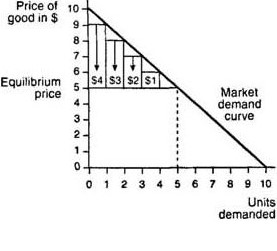
\includegraphics[width = 6cm]{consumer surplus explained.png}
        \vspace{-5.5mm}
        \caption*{Adding up individual consumer surplus's, visualized by vertical boxes, yields what we call consumer surplus. Note that this will just be the area of the triangle shown.}
    \end{figure}
\end{frame}

\begin{frame}{CS with Linear Demand Curve}
    \begin{figure}
        \centering
        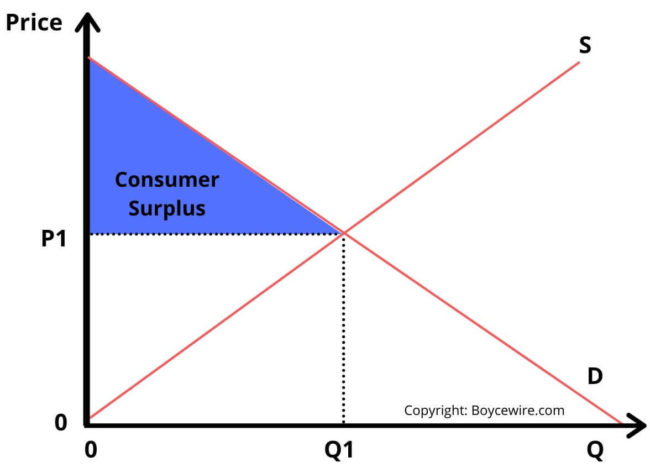
\includegraphics[width = 6.5cm]{cs triangle.jpg}
        \caption*{Here, consumer surplus is the area of the triangle, $\frac{1}{2}(b\cdot h)$ (one half base times height). In this example, $b=Q_{1}$, and $h$ would be the difference between where the demand curve intersects the $P$ axis (the $y$-intercept) and $P_{1}$.}
    \end{figure}
\end{frame}

\begin{frame}{CS with Non-Linear Demand Curve}
    \begin{figure}
        \centering
        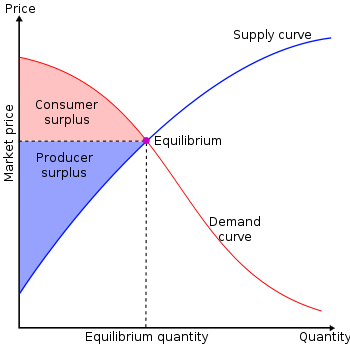
\includegraphics[width = 5cm]{curved cs.png}
        \caption*{CS with non-linear demand curve. You are not expected to provide a precise calculation of the area here; it requires calculus.}
    \end{figure}
\end{frame}

\begin{frame}{A Change in CS}
    \begin{figure}
        \centering
        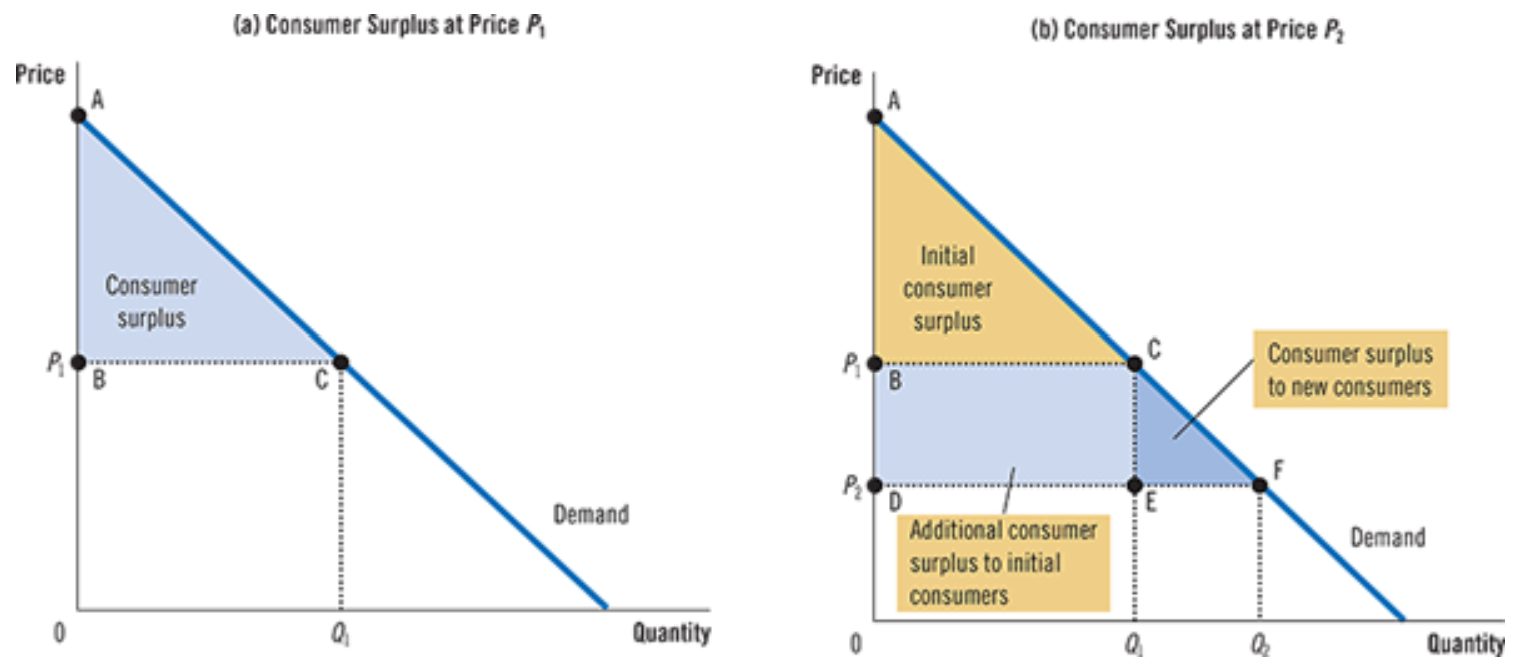
\includegraphics[width = 10cm]{change in cs.png}
        \caption*{When the price is lowered, more consumers can buy, some of which with surplus. The ones that were already buying get additional surplus, raising overall CS.}
    \end{figure}
\end{frame}


\begin{frame}{CS Exercise}
    \begin{itemize}[<+->]
        \item Reminder: the area of a triangle is $\frac{1}{2}b\cdot h$, where $b$ is the base and $h$ is the height
        \item Calculate CS in the following market
        \begin{figure}
            \centering
            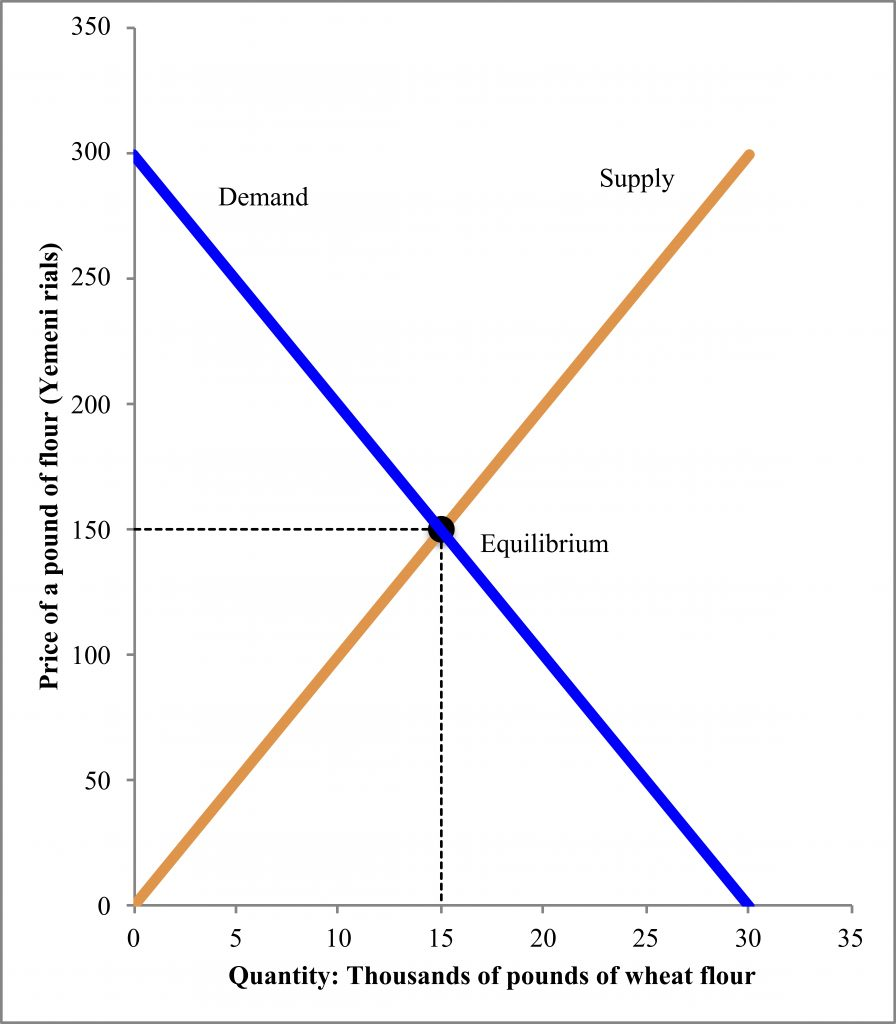
\includegraphics[width=4.5cm]{cs example.jpg}
        \end{figure}
    \end{itemize}
\end{frame}


\begin{frame}{CS Exercise Solution}
    \begin{itemize}[<+->]
        \item CS is the area of the triangle above the market price, up to the demand curve
        \item Using the figure, the base of the triangle is $15-0=15$. The height of the triangle is $300-150=150$
        \item Therefore,
        $$CS=\frac{1}{2}(15)(150)=1125$$
    \end{itemize}
\end{frame}


\begin{frame}{Bonus CS Exercise}
    \begin{itemize}[<+->]
        \item Compute CS in the figure below. You have enough information.
        \begin{figure}
            \centering
            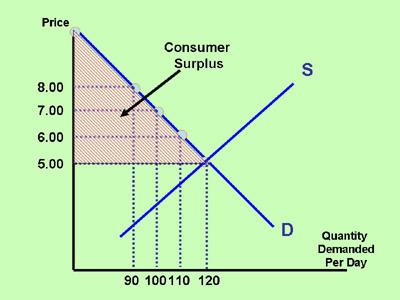
\includegraphics[width= 6cm]{cs calculation.jpg}
        \end{figure}
    \end{itemize}
\end{frame}


\begin{frame}{CS Bonus Solution}
    \begin{itemize}[<+->]
        \item Based on the figure, for every movement in price by 1, the movement in quantity is 10. So the slope of the demand curve is $-\frac{1}{10}$
        \item One way to get the $P$-intercept is to plug a known point into $P=-\frac{1}{10}Q+b$, where $b$ is the $P$-intercept (replace $P$ with $y$, if you wish, in this case. But always remember to report your final answer in terms of $P$ and $Q$, and relevant units)
        \item Using the point $(Q,P)=(5,120)$, we can compute:
        \begin{align*}
            5=-\frac{1}{10}(120)+b \ \ \implies \ \ 5=-12+b\ \ \implies\ \ b=17
        \end{align*}
        \item Therefore, the $P$-intercept is 17. Thus, using the formula for a triangle,
            \begin{align*}
            CS=\frac{1}{2}(120-0)(17-5)=60(12)=720
        \end{align*}
    \end{itemize}
\end{frame}

\section*{Relation to Mankiw}

\begin{frame}{Example à la Mankiw}
    \begin{itemize}[<+->]
        \item Suppose that you're Martin Shkreli, and you own the only copy of an exclusive Wu-Tang Clan album
        \item Suppose there are 6 buyers in the market for this album, shown with their willingness to pay:
        \begin{table}[]
            \centering
            \begin{tabular}{|c|c|c|c|c|c|c|}
            \hline
                \textbf{Consumer} & Dre & Snoop & Kendrick & J & Megan & Cardi\\
                \hline
                \thead{\textbf{WTP}\\(\$M)} & 10 & 7 & 12 & 4 & 6 & 8\\
                \hline
            \end{tabular}
        \end{table}
        \item Suppose you start the bidding at \$5M. What is the quantity demanded in the market?
        \begin{itemize}
            \item $Q_{D}=5$. Even though everyone wants the good, only 5/6 people want it for more than \$5M
        \end{itemize}
        \item As we go up in bidding price, let's say by \$1.5M each time, $\$Q_{D}$ in the market goes down, following the law of demand
            \begin{itemize}
            \item At $P=6.5$, $Q_{D}=4$, at $P=8$, $Q_{D}=3$ (barely), at $P=9.5$, $Q_{D}=2$, and at $P=11$, $Q_{D}=1$
        \end{itemize}
    \end{itemize}
\end{frame}

\begin{frame}{Example à la Mankiw (cont.)}
        \begin{table}[]
            \centering
            \begin{tabular}{|c|c|c|c|c|c|c|}
            \hline
                \textbf{Consumer} & Dre & Snoop & Kendrick & J & Megan & Cardi\\
                \hline
                \thead{\textbf{WTP}\\(\$M)} & 10 & 7 & 12 & 4 & 6 & 8\\
                \hline
            \end{tabular}
        \end{table}
    \begin{itemize}[<+->]
        \item At $P=\$11$M, the only bidder left is Kendrick. How does he feel about the transaction?
        \begin{itemize}
            \item Great! He was willing to pay \$12 million, but only had to pay \$11 million
            \item Put another way: recall that WTP is a reflection of valuation, i.e. utility. Kendrick got \$12M worth of happiness from  owning the record, but only had to pay \$1M: he has a left over \$1M worth of happiness!
            \item This leftover (or \textit{surplus}) happiness is what we are going to call Kendrick's \underline{consumer surplus}
        \end{itemize}
    \end{itemize}
\end{frame}

\begin{frame}{Remarks to Book-like Example}
    \begin{itemize}[<+->]
        \item Once again, when we limit our scope to only consumers who buy one thing, TWTP and MWTP just become WTP
        \item In order to think about a demand curve or adding up surplus's, we have to modify the example to allow more than one of the good to be sold, while still maintaining that everyone still demands at most one of the good
        \item This is better for thinking about market demand an consumer surplus informally, less good for actually doing a problem and thinking literally about a demand curve
    \end{itemize}
\end{frame}

\begin{frame}{Remarks to Book-like Example (cont.)}
    \begin{itemize}[<+->]
        \item This also generates demand curves which are not smooth, and make step-like jumps in many cases
        \begin{itemize}
            \item Recall that market demand is the sum of individual demand curves
            \item So, using the above demand information, the market demand curve would look like the following:
            \begin{figure}
                \centering
                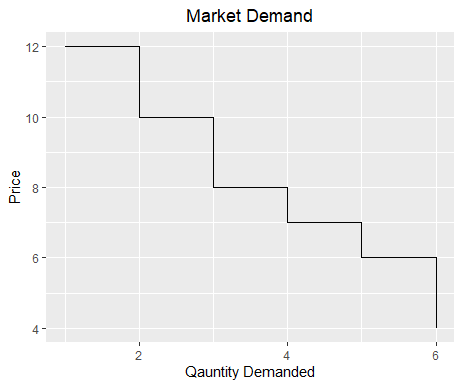
\includegraphics[width=5.5cm]{Stepwise demand plot.png}
            \end{figure}
        \end{itemize}
    \end{itemize}
\end{frame}

\begin{frame}{CS in Book-like Example}
    \begin{itemize}[<+->]
        \item With this step-wise demand curve, and allowing for the sale of more than one of the product to consumers, CS will look like
        \begin{figure}
            \centering
            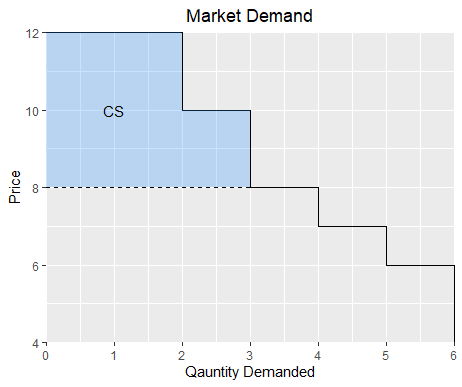
\includegraphics[width=6cm]{CSplot1.png}
            \caption*{CS when $P=8$. If you had numbers, recall that the area of a rectangle is length$\cdot$ width (or base$\cdot$ height, if you prefer to be consistent with the triangle formula).}
        \end{figure}
    \end{itemize}
\end{frame}

\begin{frame}{Change in CS: Book-like Example}
        \begin{figure}
            \centering
            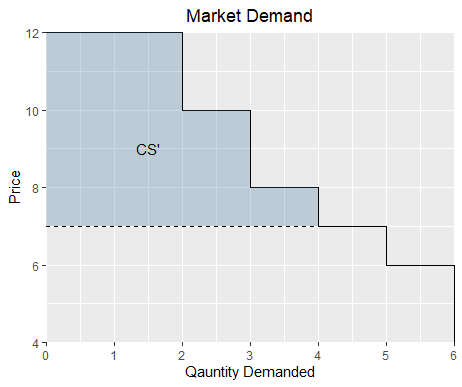
\includegraphics[width=6cm]{CSplot2.png}
            \caption*{CS when $P=7$. If you had numbers, recall that the area of a rectangle is length$\cdot$ width (or base$\cdot$ height, if you prefer to be consistent with the triangle formula).}
        \end{figure}
\end{frame}

\begin{frame}{Remarks to Book Example (cont.)}
    \begin{itemize}[<+->]
        \item Our demand curves which are not smooth, and make step-like jumps in many cases
        \begin{enumerate}
            \item<1-> If we have a lot of consumers that vary in WTP, there will be enough steps to have the graph \textit{look} smooth (this is what the book does)
            \item On the other hand, we can just say that if consumers can and will demand more than 1 unit of a good, and prices can vary continuously (as we have been doing thus far in this class), then we get a smooth demand curve anyway
        \end{enumerate}
        \item Rather than be nit-picky and specify every time, I will simply state that demand is ``a reflection of willingness to pay"
        \begin{itemize}
            \item Depending on context, keeping either of the above frameworks in mind will be helpful (a bunch of people are demanding at most 1 thing, vs some ambiguous amount of people are demanding something some amounts)
            \item Of course, in an exercise, I will try to be clear, when necessary
            \item Finally, you will have a couple homework problems that use this step-wise thinking
        \end{itemize}
    \end{itemize}
\end{frame}


\section*{Producer Surplus}

\begin{frame}{Willingness to Accept}
    \begin{itemize}[<+->]
        \item Motivating and defining producer surplus looks a lot like consumer surplus
        \item Producers have a ``willingness to accept": the minimum price that a producer will take in order to sell a product
        \item A producer's \underline{\textbf{Total Willingness to Accept}} (TWTA) is the minimum amount a producer will take in order to sell a specific quantity of a good
        \item A consumer's \underline{\textbf{Marginal Willingness to Accept}} (MWTA) is the  minimum amount a producer will take to sell the \underline{next}\footnote{\vspace{1mm} Again, ``last", depending on context} unit of a good
    \end{itemize}
\end{frame}

\begin{frame}{WTA Schedule}
    \begin{itemize}[<+->]
        \item Just as with the consumer, a we can assign a WTA schedule for a producer:
        \begin{table}
        \begin{tabular}{ccc}
                \thead{\textbf{Quantity Supplied}\\ (\# Apples)} & \thead{\textbf{Total WTA}\\ (Dollars)} & \thead{\textbf{Marginal WTA}\\ (Dollars)} \\ 
                \hline
                0 & 0.00 & {--} \\
                1 & 14.00 & {14.00} \\
                2 & 20.00 & {6.00} \\
                3 & {25.00} & 5.00 \\
                4 & 29.00 & {4.00}\\
                5 & {32.00} & 3.00\\
                6 & {34.00} & 2.00\\
                7 & 35.00 & {1.00}\\
                8 & {36.00} & 1.00 \\
                9 & 42.00 & {6.00}
                \end{tabular}
        \end{table}
        \item This induces a supply curve for the producer
    \end{itemize}
\end{frame}

\begin{frame}{Producer Surplus Motivation}
    \begin{itemize}[<+->]
        \item Suppose it only costs Caspian \$2 to make a breakfast pita, so they are willing to accept \$2
        \item However, the market price of a breakfast pita is \$4
        \item Caspian gets a ``bonus" from selling the pita at a higher price than it's worth -- in this case, profit
        \footnote{One could conceive that a producer is endowed with some goods, and still has some minimum price they are willing to sell at. Thus, producer surplus need not always equal profit}
        \item Other sellers of breakfast pitas may be willing to accept \$1, some \$3.50, etc. 
        \item Each of them gets an individual surplus from getting a ``deal" on their pita, as long as their WTA is low enough to sell the product $(\leq \$4)$
        \item If we add these surplus values up, for everyone who sold the pita, then we get what we call the \underline{producer surplus}
    \end{itemize}
\end{frame}

\begin{frame}{Producer Surplus Definition}
    \begin{itemize}[<+->]
        \item \underline{\textit{[Individual] Producer Surplus}} is the difference between a seller's WTA and the price they actually sell for \footnote{Throughout: assuming this value is positive, i.e. assuming they sold the product}
        \item \underline{\textbf{Producer Surplus}} is the the sum of all individual producer surplus's; i.e., it is the area between the WTA reflected by the market supply curve, and the price at which the good was sold
        \item Producer surplus is our measure for the overall utility (often thought of as profit), or ``welfare", on the seller's side of the market
        \item Selling a product gives the producer happiness through money, but working to produce and parting with the product took away some happiness. Whatever is leftover is the economic well-being of producers in the market
    \end{itemize}
\end{frame}

\begin{frame}{Producer Surplus Comments}
    \begin{itemize}[<+->]
        \item Just as before, Mankiw does all of this in terms of sellers who supply at most one of a good, generating step-wise supply curves
        \begin{itemize}
            \item I will leave this up to you to read
        \end{itemize}
        \item To allow for generality, I will simply state that supply is a reflection of willingness to accept\footnote{Later, it will be a reflection of marginal costs to the producer}
        \item For now, the \underline{\textbf{Total Surplus}} in the market is the sum of producer and consumer surplus
    \end{itemize}
\end{frame}


\begin{frame}{Graphical Representation of PS}
    \begin{figure}
        \centering
        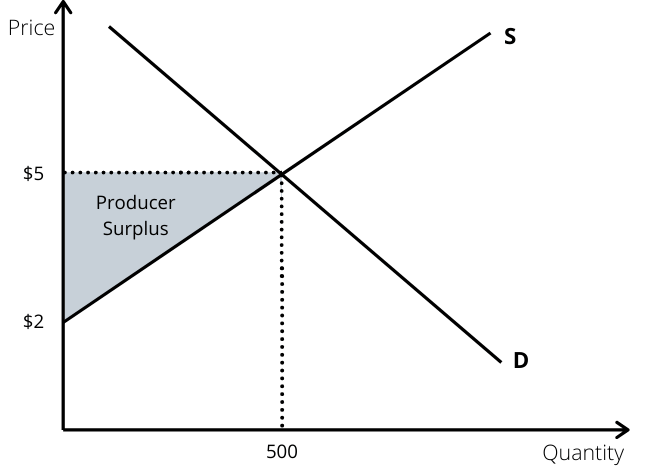
\includegraphics[width=7cm]{ps graphically.png}
        \caption*{PS is the area enclosed between the price, the price axis, and the supply line (in the first quadrant)}
    \end{figure}
\end{frame}

\begin{frame}{Change in PS}
    \begin{figure}
        \centering
        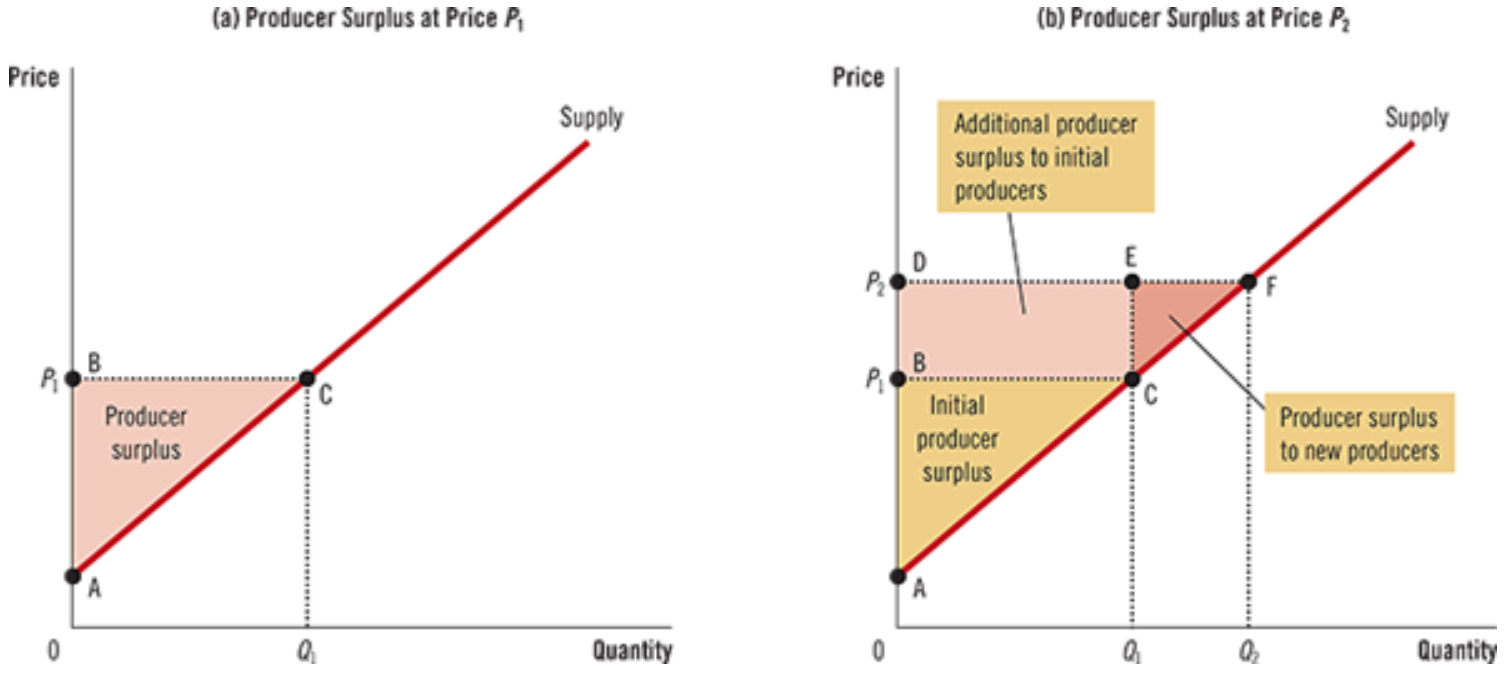
\includegraphics[width=10cm]{change in ps.png}
        \caption*{When the price is raised, more producers will sell, some of whom get surplus for their sale. The ones that were already buying get additional surplus, raising overall PS}
    \end{figure}
\end{frame}

\begin{frame}{TS With Curved Supply and Demand}
    \begin{figure}
        \centering
        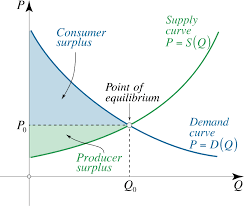
\includegraphics[width=7cm]{Supply with curved lines.png}
    \end{figure}
\end{frame}

\begin{frame}{Total Surplus Exercise}
    \begin{itemize}
        \item Compute total surplus in the following economy
    \begin{figure}
        \centering
        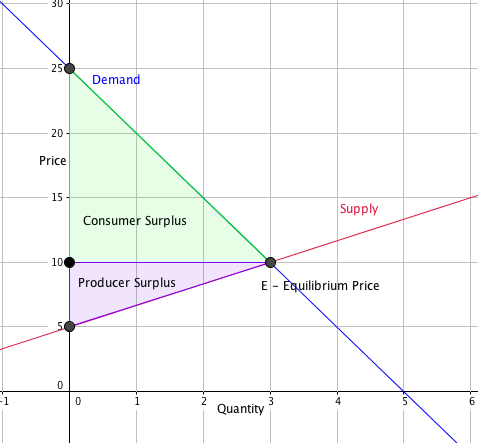
\includegraphics[width=6cm]{ts example.png}
    \end{figure}
    \end{itemize}
\end{frame}

\begin{frame}{TS Solution}
    \begin{itemize}
        \item Consumer surplus is given by 
        $$CS=\frac{1}{2}(3)(25-10)=\frac{1}{2}(3)(15)=\frac{1}{2}(45)=22.5$$
        \item Producer Surplus is given by
        $$PS=\frac{1}{2}(3)(10-5)=\frac{1}{2}(3)(5)=\frac{1}{2}(15)=7.5$$
        \item Therefore, 
        $$TS=CS+PS=22.5+7.5=30$$
    \end{itemize}
\end{frame}


\end{document}